%% Standalone source of one report figure. Rebuild: pdflatex -output-directory=.. fig-05-dataset-build.tex
\documentclass[11pt]{standalone}
\usepackage[T1]{fontenc}
\usepackage[utf8]{inputenc}
\usepackage{lmodern}
\usepackage{microtype}
\usepackage{amsmath,amssymb}
\usepackage{xcolor}
\usepackage{tikz}
\usetikzlibrary{arrows.meta,positioning,shapes.geometric,fit,calc,backgrounds}
\usepackage{pgfplots}
\usepackage{pgfplotstable}
\pgfplotsset{compat=1.18}
\setlength{\textwidth}{472.31595pt}  %% = the report's text width, so widths given in \textwidth match
\definecolor{gmblue}{HTML}{0B3D6E}
\definecolor{gmok}{HTML}{1E7B34}
\definecolor{gmwarn}{HTML}{B35C00}
\definecolor{gmbad}{HTML}{A32020}
\definecolor{gmgrey}{HTML}{5A5F66}
\definecolor{gmlight}{HTML}{EEF3F8}
\definecolor{gmteal}{HTML}{1B7A8C}
\newcommand{\done}{\textcolor{gmok}{\textbf{Done}}}
\newcommand{\partly}{\textcolor{gmwarn}{\textbf{Partly}}}
\newcommand{\pending}{\textcolor{gmbad}{\textbf{Pending}}}
\newcommand{\pass}{\textcolor{gmok}{\textbf{PASS}}}
\newcommand{\fail}{\textcolor{gmbad}{\textbf{FAIL}}}
\newcommand{\code}[1]{\texttt{\small #1}}
\newcommand{\INR}{INR~}
\newcommand{\gbar}[5]{\fill[#5] (#1,-#3+0.32) rectangle (#2,-#3-0.32);
  \node[anchor=east,font=\scriptsize] at (-0.3,-#3) {#4};}

\tikzset{
  box/.style={draw=gmblue, rounded corners=3pt, fill=gmlight, align=center, font=\small, inner sep=5pt,
              minimum height=9mm},
  gstep/.style={draw=gmblue, rounded corners=3pt, fill=white, align=center, font=\footnotesize, inner sep=4pt,
               text width=27mm, minimum height=11mm},
  st/.style={draw=gmblue, rounded corners=6pt, fill=gmlight, font=\scriptsize\ttfamily, inner sep=3pt,
             minimum height=6mm},
  arr/.style={-{Stealth[length=2.2mm]}, thick, gmblue},
  darr/.style={-{Stealth[length=2mm]}, gmgrey, dashed},
}

\begin{document}
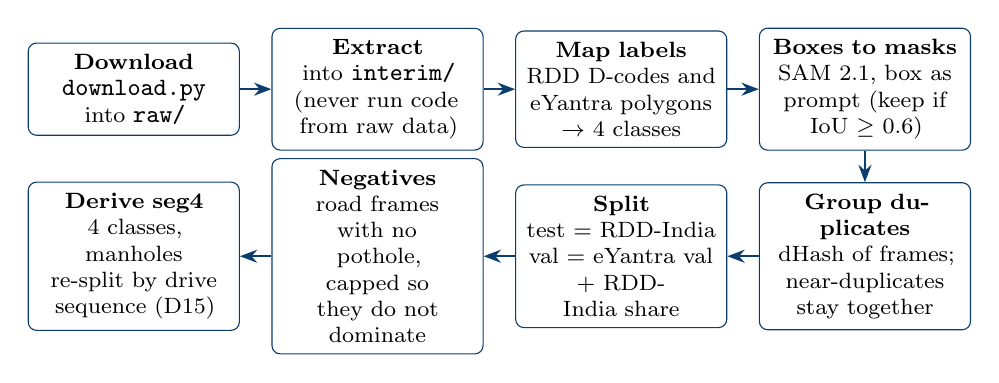
\begin{tikzpicture}[node distance=4mm and 4mm, every node/.style={gstep, text width=24mm}]
  \node (dl) {\textbf{Download}\\\code{download.py}\\into \code{raw/}};
  \node[right=of dl] (ex) {\textbf{Extract}\\into \code{interim/}\\(never run code\\from raw data)};
  \node[right=of ex] (map) {\textbf{Map labels}\\RDD D-codes and\\eYantra polygons\\$\rightarrow$ 4 classes};
  \node[right=of map] (sam) {\textbf{Boxes to masks}\\SAM 2.1, box as\\prompt (keep if\\IoU $\ge$ 0.6)};
  \node[below=of sam] (dup) {\textbf{Group duplicates}\\dHash of frames;\\near-duplicates\\stay together};
  \node[left=of dup] (spl) {\textbf{Split}\\test = RDD-India\\val = eYantra val\\+ RDD-India share};
  \node[left=of spl] (neg) {\textbf{Negatives}\\road frames with no\\pothole, capped so\\they do not dominate};
  \node[left=of neg] (der) {\textbf{Derive seg4}\\4 classes, manholes\\re-split by drive\\sequence (D15)};
  \draw[arr] (dl)--(ex); \draw[arr] (ex)--(map); \draw[arr] (map)--(sam); \draw[arr] (sam)--(dup);
  \draw[arr] (dup)--(spl); \draw[arr] (spl)--(neg); \draw[arr] (neg)--(der);
\end{tikzpicture}
\end{document}
